\documentclass[tikz,border=2pt]{standalone}
\usepackage{amsmath}
\usepackage{newtxtext,newtxmath} % Times-like to match IEEEtran
\usetikzlibrary{arrows.meta,positioning,calc,fit,shapes.multipart,decorations.pathmorphing}
\tikzset{>=Latex, line/.style={line width=0.8pt}, box/.style={draw, rounded corners=2pt, minimum width=28mm, minimum height=12mm, align=center},
note/.style={font=\footnotesize}}

\begin{document}
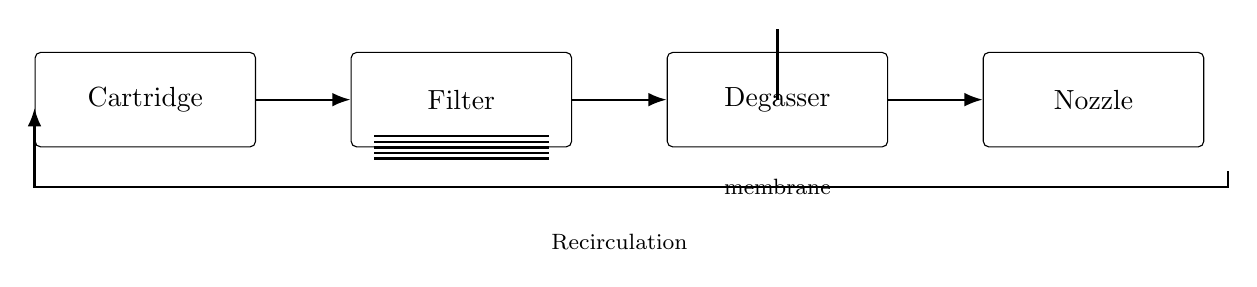
\begin{tikzpicture}[node distance=12mm]
\node[box] (cart) {Cartridge};
\node[box, right=of cart] (filter) {Filter};
\node[box, right=of filter] (degas) {Degasser};
\node[box, right=of degas] (nozzle) {Nozzle};

\draw[->,line] (cart) -- (filter);
\draw[->,line] (filter) -- (degas);
\draw[->,line] (degas) -- (nozzle);

% filter mesh
\foreach \y in {-4,-2,0,2,4} {
  \draw[line] ($(filter.south west)+(3mm, \y pt)$) -- ($(filter.south east)+(-3mm, \y pt)$);
}

% membrane line in degasser
\draw[line] ($(degas.south)!0.5!(degas.north)$) -- ++(0,0.9);
\node[note] at ($(degas.south)+(0,-5mm)$) {membrane};

% recirculation loop
\draw[line] (nozzle.south east) ++(3mm,-3mm) |- ($(cart.south)-(0,5mm)$) -| (cart.south west);
\draw[->,line] ($(cart.south west)$) -- ++(0,5mm);
\node[note] at ($(cart.south)!0.5!(nozzle.south)+(0,-12mm)$) {Recirculation};
\end{tikzpicture}
\end{document}
